\chapter{Organizacja pracy}



Aby dobrze zorganizować pracę nad projektem, odbywały się spotkania w~obrębie grupy projektowej. Miały one na celu kreatywne rozwiązywanie bieżących problemów, występujących podczas tworzenia aplikacji. 

Raz w~tygodniu odbywały się także spotkania na terenie uczelni, w~których brali udział:
\begin{itemize}
\item Promotor
\item Grupa TWO
\item Zespół tworzący projekt
\end{itemize}

\paragraph{}
Na spotkaniu poruszane były bieżące problemy dotyczące aplikacji, oraz weryfikowany był postęp prac przez grupę TWO. Weryfikacja postępu prac polegała na sprawdzeniu, czy zostały poprawnie wykonane przydzielone zadania w~ramach przyrostu. Przyrost to zbiór zadań jakie należało wykonać do następnego przyrostu. Zwykle taki przyrost trwał około jednego miesiąca. Dzięki temu czas realizacji pracy był zgodny z~tym zawartym w~harmonogramie projektu. W ramach spotkania prowadzone były także konsultacje z~promotorem.

Do sprawnej organizacji pracy wykorzystane zostały darmowe narzędzia dostępne w~Internecie, przeznaczone do tego typu potrzeb. Były to trzy aplikacje:
\begin{itemize}
\item GitHub
\item Trello
\item Komunikator dostępny w~portalu Facebook
\end{itemize}

\section{GitHub}
GitHub to internetowy serwis hostingowy, wykorzystywany do prowadzenia projektów programistycznych wykorzystujących system kontroli wersji Git. 

Każda wersja aplikacji udostępniana była pozostałym członkom grupy projektowej poprzez ten serwis. Dzięki temu możliwa była synchronizacja fragmentów aplikacji stworzonych przez każdego członka grupy. Za pośrednictwem serwisu każdy członek grupy miał ponadto możliwość śledzenia na bieżąco postępów pracy oraz dostępu do najnowszej wersji projektu. 
\begin{figure}[h]
	\centering
	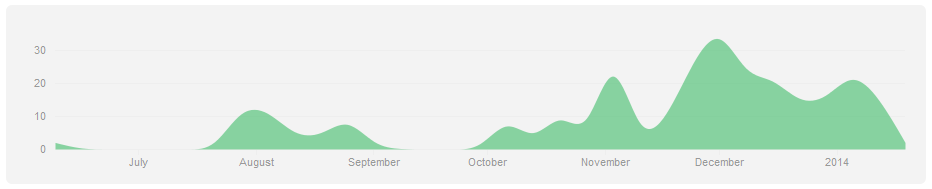
\includegraphics[width=1.00\textwidth]{images/git.png}
	\caption{Aktywność grupy projektowej w~serwisie GitHub}
\end{figure}

Diagram przedstawia aktywność grupy projektowej w~serwisie. Wartością na wykresie jest liczba zmian dokonanych w~projekcie, które zostały udostępnione pozostałym członkom na przestrzeni całego okresu tworzenia aplikacji. 

\section{Trello}
Trello to aplikacja, której zadaniem jest usprawnienie organizacji pracy poprzez wygodne zarządzanie oraz przydzielanie zadań poszczególnym członkom projektu. Trello jest aplikacją umożliwiającą tworzenie list ze zbiorami zadań. Na każdej takiej liście jest możliwość dodania karty, która zawiera opis zadania do wykonania. Do tych kart można także przypisać etykiety z nazwą użytkowników, którzy będą wykonywać dane zadanie, a~także załączyć pliki,  na przykład graficzne, w~celu zobrazowania danego zadania. Rozpoczęcie pracy z~Trello  to kwestia chwili. Proces rejestracji trwa moment, a~sama aplikacja jest bardzo prosta w~użytkowaniu, ze względu na intuicyjny interfejs użytkownika. Cechy te sprawiają, że jest to bardzo wygodny organizer pracy i~dlatego został on wykorzystany przy tworzeniu projektu. Grupa TWO za pomocą tej aplikacji miała możliwość dodawania nowych zadań oraz nadawania im priorytetów. Od momentu rozpoczęcia pracy z~aplikacją, mieli oni wygodny dostęp do informacji opisujących stan zaawansowania prac nad przydzielonymi zadaniami. Umożliwiało im to wyznaczanie na bieżąco kolejnych zadań, zgodnie z~harmonogramem prac nad projektem. Same zadania przydzielane były poszczególnym członkom grupy projektowej przez nich samych. 

\begin{figure}[H]
	\centering
	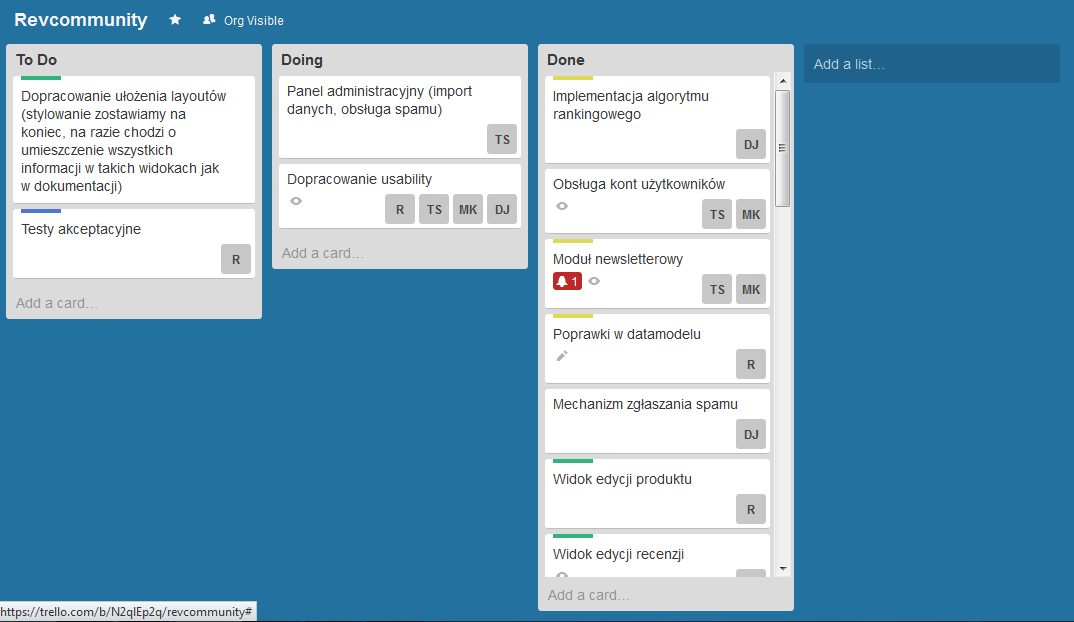
\includegraphics[width=1.00\textwidth]{images/trello.png}
	\caption{Interfejs użytkownika w~serwisie Trello}
	\label{fig:trello}
\end{figure}

Rysunek \ref{fig:trello} przedstawia interfejs użytkownika w serwisie Trello. Znajdują się na nim trzy listy z grupami zadań.

\begin{itemize}
\item ,,To Do'' zawiera wszystkie zadania, które nie zostały jeszcze wykonane,
\item ,,Doing'' to zbiór zadań, które są aktualnie wykonywane,
\item ,,Done'' to grupa zadań, które zostały ukończone.
\end{itemize}


Kolorowe etykiety przedstawiają priorytet dla konkretnego zadania. Kolor żółty to zadania z~najwyższym priorytetem a~kolor niebieski to zadania o~najniższym priorytecie. Przy każdym zadaniu umieszczone są skrócone nazwy kont użytkowników w~serwisie, którym zostało przydzielone to zadanie. 
Serwis umożliwił wygodne oraz przejrzyste zarządzanie zadaniami związanymi z~projektem.

\section{Komunikator dostępny w~portalu Facebook}
Facebook jest serwisem społecznościowym, w~ramach którego zarejestrowani użytkownicy mogą tworzyć sieci i~grupy, dzielić się wiadomościami, zdjęciami i~filmami, a~także korzystać z~aplikacji, które są własnością Facebook.\cite{face} Do komunikacji w~projekcie została wykorzystana tak zwana grupa w~serwisie Facebook. Grupa  jest to zamknięta przestrzeń przeznaczona dla kilku osób, które chcą się komunikować w~łatwy sposób i~przy okazji zapewnić sobie prywatność. Dzięki temu zapewniony był stały i~szybki kontakt pomiędzy grupą TWO a~grupą projektową. Wszystkie pojawiające się problemy i~wątpliwości podczas tworzenia aplikacji konsultowane były na forum grupy. Najczęściej poruszanymi tematami były:

\begin{itemize}
\item Implementacja konkretnej funkcjonalności,
\item Dokładne omówienie zadań przydzielonych w~serwisie Trello,
\item Rozdzielenie przydzielonych zadań pomiędzy członków grupy projektowej.
\end{itemize}
\paragraph{}


Na forum grupy poruszane były także kwestie związane z~organizacją cotygodniowych spotkań, które miały na celu prezentację postępu pracy nad projektem. Korzystanie z~tej funkcjonalności serwisu Facebook zapewniło sprawną pracę nad projektem. 